\section{RESULTS}
\subsection{CO EMISSION}

\begin{figure*}[htbp]
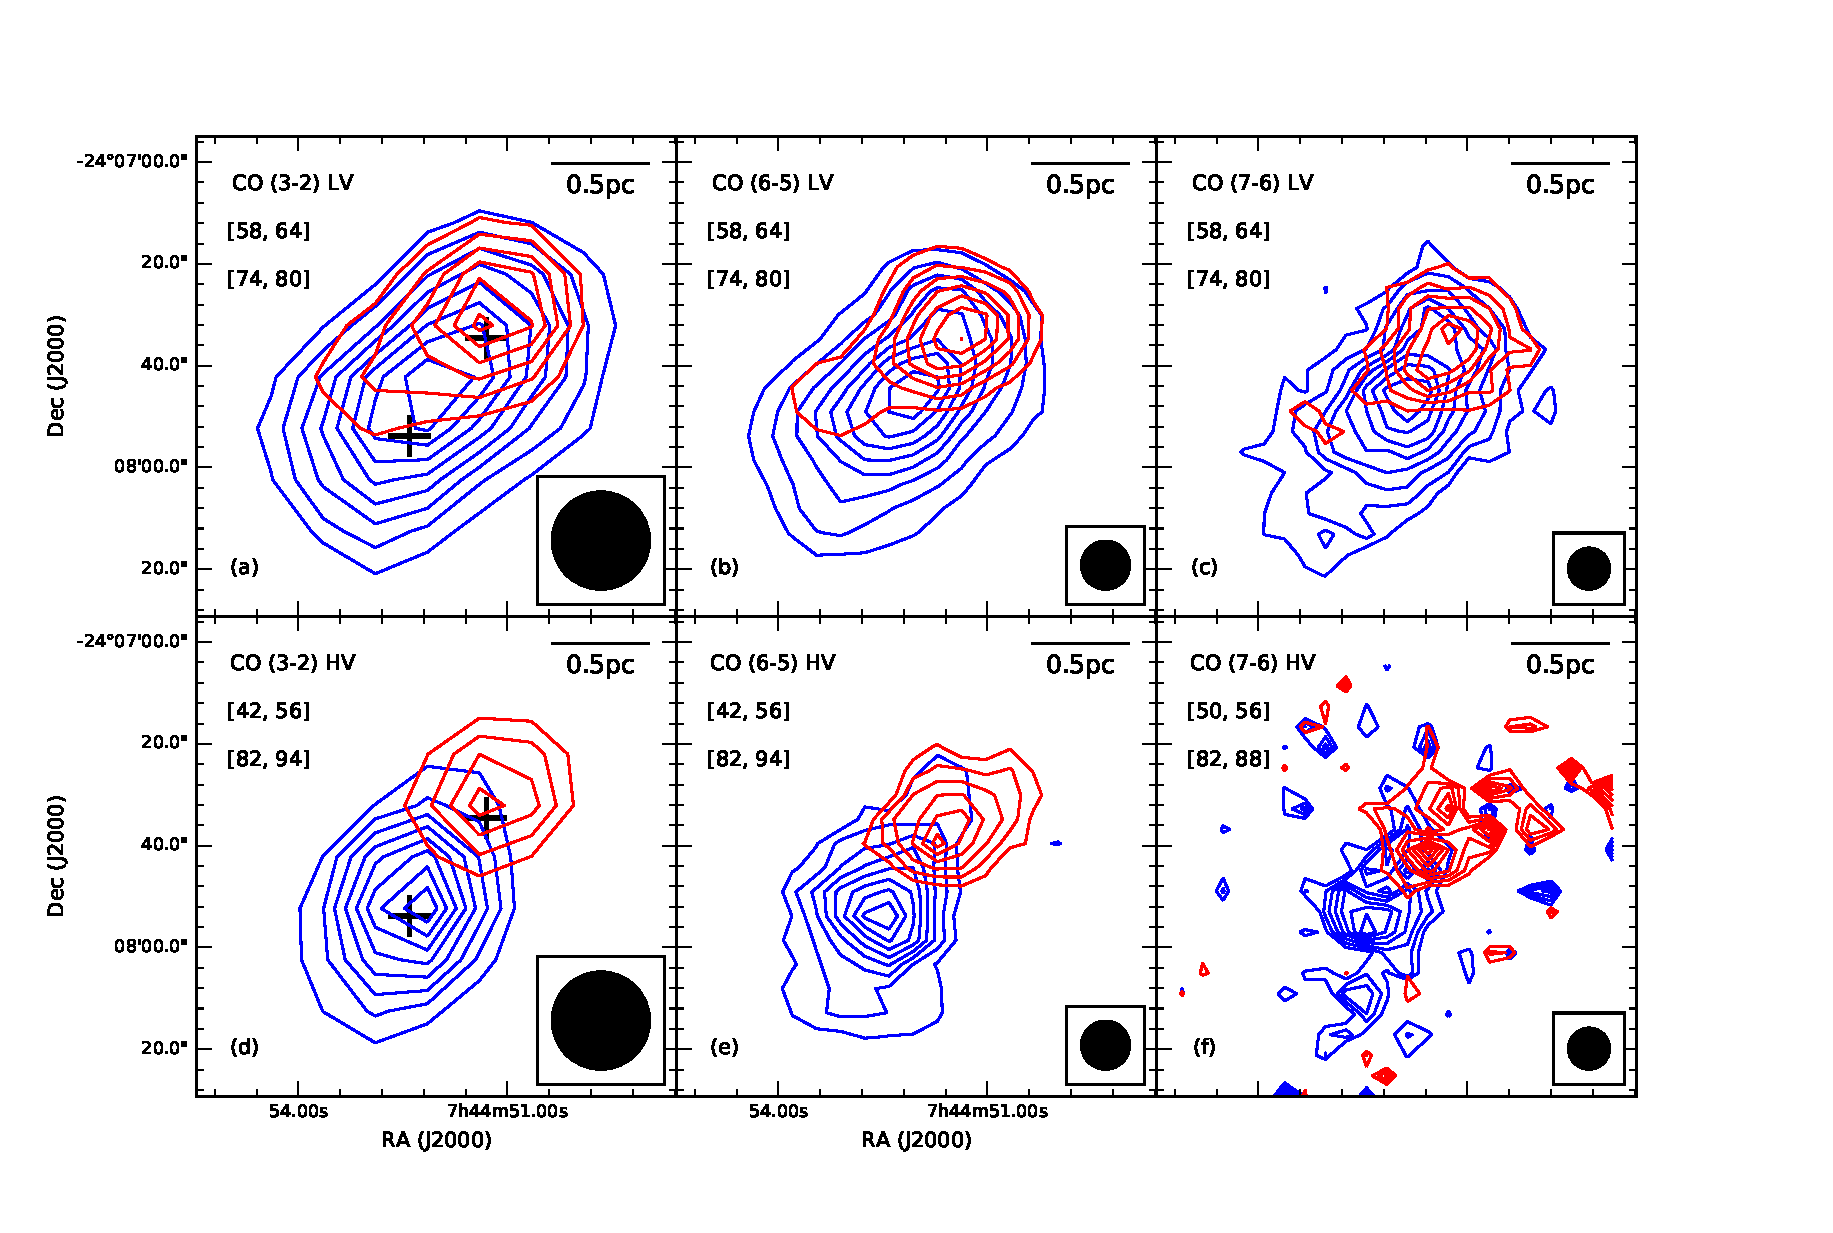
\includegraphics[scale=.60]{./fig/ori_contour.eps}
\caption{(a)-(c) Low-velocity emission of CO J = (3-2), (6-5), (7-6) lines, with velocity range 58 to 64 km s$^{-1} $ and 74 to 80 km s$^{-1}$ for the blueshifted lobe (blue) and the redshifted lobe (red); (d)-(e) High-velocity emission of CO J = (3-2), (6-5) lines, with velocity range 42 to 56 km s$^{-1} $ and 82 to 94 km s$^{-1}$ for the blueshifted lobe (blue) and  the redshifted lobe (red); (f) High-velocity CO J = (7-6) emission, with velocity range 50 to 56 km s$^{-1} $ and 82 to 88 km s$^{-1}$ for the blueshifted lobe (blue) and  the redshifted lobe (red). For (a)-(e), the contour levels are starting from 20\% and at steps of 10\%. For (f), the contour levels are starting from 30\% and at steps of 10\%. The central stars mark the position of the millimeter sources detected by \citet{2009ApJ...696...66Q}. The beam size is shown in the lower right corner of each panel.  \label{fig1}}
\end{figure*}

Figure \ref{fig1} shows maps of the integrated low-velocity (LV) and high-velocity (HV) blueshifted and redshifted emissions of CO J = (3-2), (6-5), (7-6) lines. For comparison, we integrate the LV and HV line wings of CO (3-2) and CO (6-5), as well as CO (7-6) LV emission, with the same velocity range as \citet{2009ApJ...696...66Q} Figure 2 (a) and Figure 2 (b), which is 58 to 64 km s$^{-1} $ and 74 to 80 km s$^{-1}$ for the LV blueshifted lobe and redshifted lobe, 42 to 56 km s$^{-1} $ and 82 to 94 km s$^{-1}$ for the HV blueshifted lobe and redshifted lobe. As CO (7-6) observation is less sensitive than observations of CO (3-2) and CO (6-5), we integrate the HV emission of CO (7-6) with 50 to 56 km s$^{-1} $ for the blueshifted lobe and 82 to 88 km s$^{-1}$ for the redshifted lobe, to exclude channels which are dominated by noise. 
For CO J = (3-2) and (6-5) emissions, a low-velocity and high-velocity prominent bipolar outflow is detected at position angle (PA) $\approx$ 131${\degr}$, along with a low-veloticy weaker component detected at PA $\approx$ 101${\degr}$. However, the weaker outflow is not clearly seen in CO (7-6). It could result from the limited sensitivity of CO (7-6) observation. And, due to lower resolution of our CO J = (3-2), (6-5), (7-6) observations, we don't see the wide-angle structure reported by \citet{2009ApJ...696...66Q}.

\subsection{LINE RATIOS}
With multi transition CO lines observation, it is feasible to estimate the physical parameters of the outflowing and investigate their velocity dependence by means of statistical-equilibrium calculations. For a proper comparison, we reconstructed CO (2-1), (6-5) and (7-6) data to the same spatial resolution of CO (3-2), which is 19${\arcsec}$.16. To reduce the noise level, we resampled the spectra of four CO lines to a resolution of 2 km s$^{-1}$. Then we measured the main beam temperature ratios of the four transitions toward the peak of the blueshifted and redshifted lobes (marked as two crosses in Figure \ref{fig1}). We adopted the cloud velocity (v$_{\textup{cloud}}$) from \citet{2003A&A...412..175K}, which is about 67.5 km s$^{-1}$ with respect to the local standard of rest. Figure \ref{fig2} shows the ratio-velocity distributions of the blueshifted gas and redshifted gas. The plot exhibits that all line ratios ((7-6)/(6-5), (6-5)/(3-2), (6-5)/(2-1)) keep almost unchanged with the increase of outflow velocity, thus indicating the homogenousness within the outflowing gas.

\begin{figure}[tbp]
\plotone{./fig/ratio.eps}
\caption{Ratios of main beam temperature of different CO lines versus outflowing gas velocity, as observed towards the blueshifted lobe (blue symbols) and the redshifted lobe (red symbols). The $V_{\textup{outflow}}$ shown here is the gas velocity with respect to the cloud velocity ($v_{\textup{cloud}}$): $V_{\textup{outflow}}$ = $\mid$ $v_{\textup{observed}}$ - $v_{\textup{cloud}}\mid$, where $v_{\textup{observed}}$ is the observed gas velocity. \label{fig2}}
\end{figure}

\subsection{PHYSICAL PROPERTY ANALYSIS}
We performed LVG analysis with the radiative transfer code RADEX developed by \citet{2007A&A...468..627V}. The simulation constructs a large grid of non-LTE models with three parameters: gas density ($n_{\textup{H}_2}$), kinetic temperature ($T_{\textup{kin}}$), and the ratio between column density and line width ($N_{\textup{CO}}$/$\Delta V$). Considering of the velocity resolution of our observations, we fix $\Delta V$ to 2 km s$^{-1}$. Each model gives the prediction of the brightness temperature ($T_\textup{b}$) of different CO transitions. With CO line datas resampled and reconstructed, we measured main beam temperature ($T_{\textup{mb}}$) of the four CO lines extracted at the peak position of the blue lobe and red lobe (marked as two crosses in Figure \ref{fig1}). To compare the simulated $T_\textup{b}$ with our measured $T_{\textup{mb}}$, we need to consider about the beam dilution, as $T_{\textup{mb}}$ is related to $T_\textup{b}$:
\begin{equation}
T_{\textup{mb}} = \frac{\Omega_{\textup{s}}^2}{\Omega_{\textup{s}}^2+\Omega_{\textup{mb}}^2}\times T_\textup{b} = \eta_{\textup{b}} \times T_\textup{b},
\end{equation}
where $\Omega_{\textup{s}}^2$ and $\Omega_{\textup{mb}}^2$ are the source size and the beam size in arcsec, and $\eta_{\textup{\textup{b}}}$ is the beam filling factor. Given the complex structures of G240 outflow at higher resolution \citep{2009ApJ...696...66Q}, we can't get a good estimate of the source size. Then the beam filling factors are assumed to be the same for all transitions, and fixed to 1, during our analysis. Thus, the derived physical parameters of the gas are beam-averaged values. We further discuss how the beam dilution affect our results in the belowing part of this section.

We report the results from a $\chi^2_{\textup{red}}$ fitting. $\chi^2_{\textup{red}}$ is the reduced $\chi^2$: 
\begin{equation}
\chi^2_{\textup{red}} = \frac{1}{N - n} \sum_{i=1}^{4}(I_o - I_m)^2/\sigma^2,
\end{equation}
where $N$ is the number of observed intensities, $n$ the number of fitted parameters, $I_\textup{o}$ the observed intensity, $I_\textup{m}$ the modelled intensity, and $\sigma$, the uncertainty of the observed intensity. With four lines observations and three simulation parameters, our fitting has one degrees of freedom. Considering the calibration error and pointing accuracy of our CO observations, we set the intensity uncertainty of CO (2-1), CO (3-2), CO (6-5), CO (7-6) to 0.15, 0.2, 0.25, 0.3 respectively. The best fit is then obtained by minimizing the $\chi^2_{\textup{red}}$ between the observed and modelled data using the Levenberg-Marquardt method \citep{1992nrfa.book.....P}. However, in velocities where no CO (7-6) emission is detected, the best fit is obtained by minimizing $\chi^2$ instead of $\chi^2_{\textup{red}}$. Then we found the best fitting result at most velocities has a $\chi^2_{\textup{red}}$ less than 1, indicating that we might be a bit conservative at the intensity uncertainty. So we divided the intensity uncertainties by a appropriate factor to make $\chi^2_{\textup{red}}$ approach 1 at most velocities. At some velocities, the $\chi_{\textup{red}}^2$ remains much less than 1 even after our adjustment of intensity uncertainty, which can accounts for the anomaly high upper limits of gas temperature at these velocities in Figure \ref{fig4a}. 

\begin{figure}[tbp]
\centering
\subfigure[]{
\begin{minipage}[b]{0.5\textwidth}
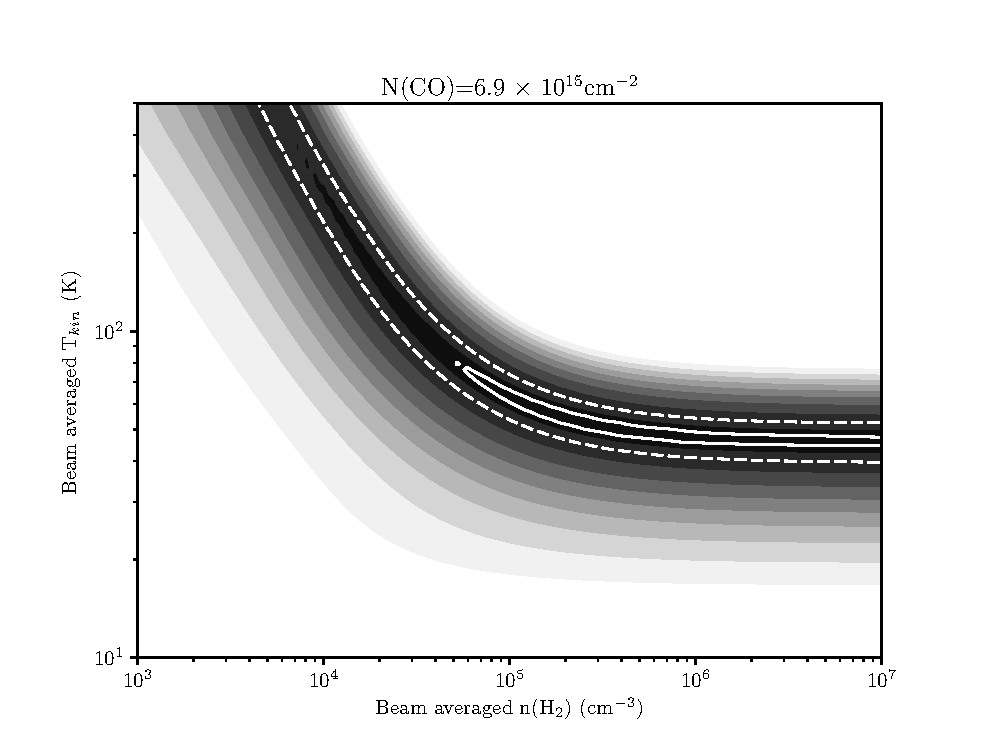
\includegraphics[width=1\textwidth]{./fig/chiimage_nco_paper.eps}
\label{fig3a}
\end{minipage}
}
\subfigure[]{
\begin{minipage}[b]{0.5\textwidth}
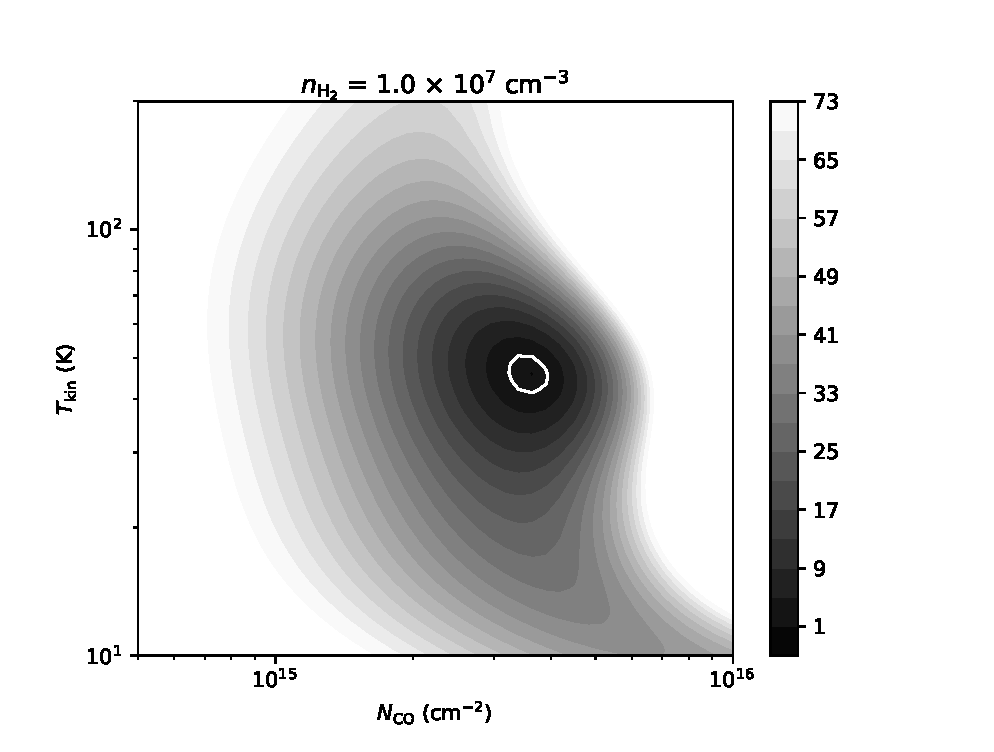
\includegraphics[width=1\textwidth]{./fig/chiimage_nh2_paper.eps}
\label{fig3b}
\end{minipage}
}
\subfigure[]{
\begin{minipage}[b]{0.5\textwidth}
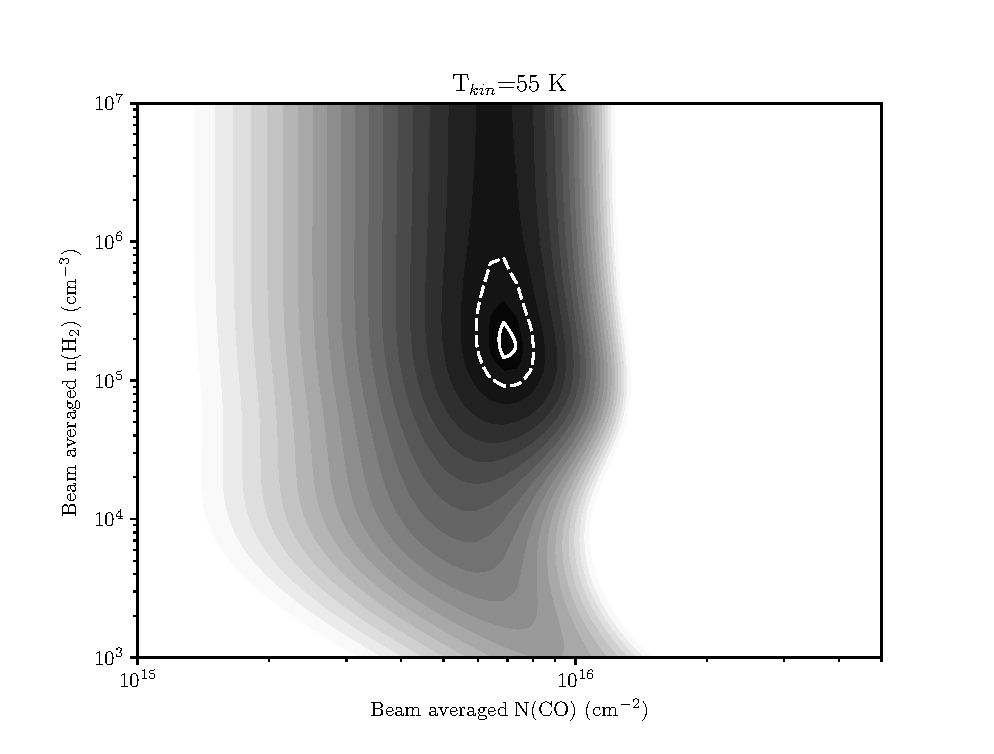
\includegraphics[width=1\textwidth]{./fig/chiimage_tkin_paper.eps}
\label{fig3c}
\end{minipage}
}
\caption{The $\chi_{\textup{red}}^2$ distribution for G240 outflow at 58 km s$^{-1}$ in the (a) [$T$, $n$], (b) [$T$, $N$], (c) [$n$, $N$] planes, with all other parameters fixed to the parameters of the best fitting results at this velocity. Solid contours and dashed contours show the 1$\sigma$ and 3$\sigma$ confidence levels respectively. \label{fig3}}
\end{figure}

In Figure \ref{fig3}, we show cuts in the $\chi_{\textup{red}}^2$ along the [$T$, $n$], [$T$, $N$], [$n$, $N$] planes for 58 km s$^{-1}$ as examples of the $\chi_{\textup{red}}^2$ distribution, with all other parameters fixed to  the parameters of the best fitting results at this velocity. The $\chi_{\textup{red}}^2$ distribution in [$T$, $n$], [$T$, $N$] planes is well behaved, with only one minimum, as shown in Figure \ref{fig3b} and Figure \ref{fig3c}. However, Figure \ref{fig3a} shows that the gas might be thermalised and no upper limits to the density could be derived. The $\chi_{\textup{red}}^2$ distribution behaves similarly at other velocities. 

\begin{figure}[htbp]
\centering
\subfigure[]{
\begin{minipage}[b]{0.5\textwidth}
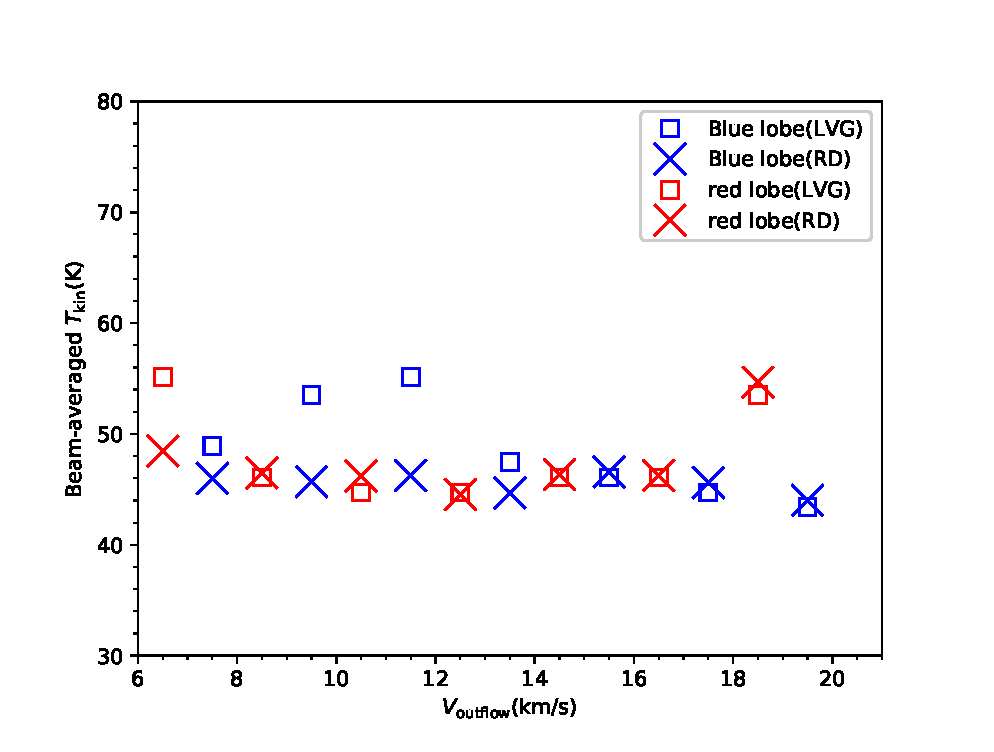
\includegraphics[width=1\textwidth]{./fig/tv_paper.eps}
\label{fig4a}
\end{minipage}
}
\subfigure[]{
\begin{minipage}[b]{0.5\textwidth}
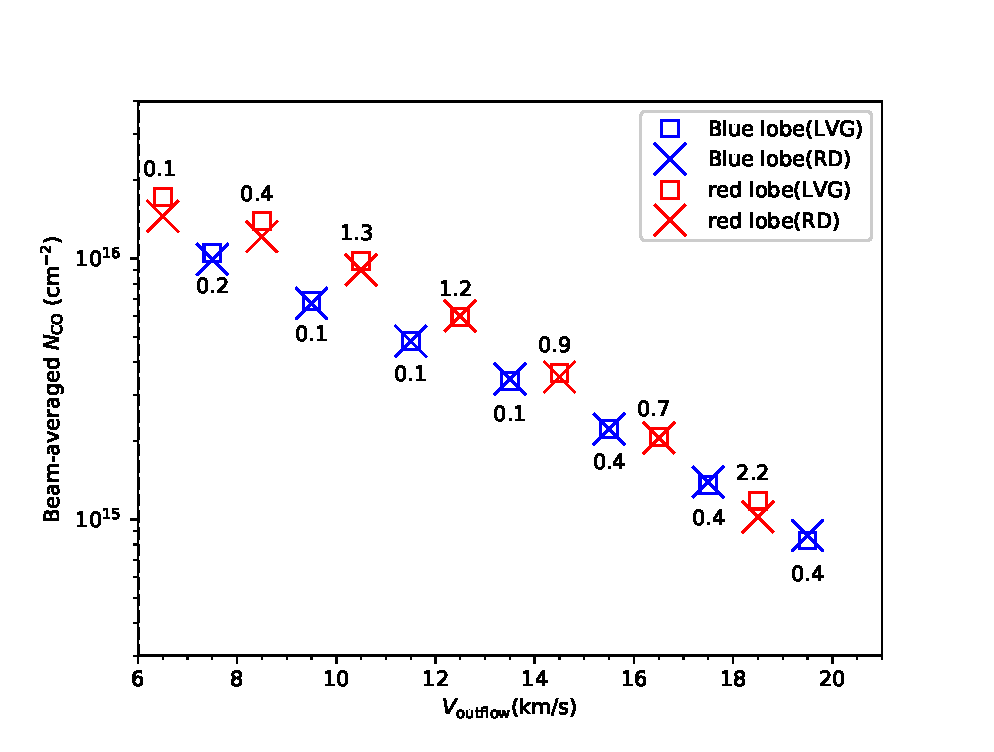
\includegraphics[width=1\textwidth]{./fig/Nv_paper.eps}
\label{fig4b}
\end{minipage}
}
\caption{$T$-$V$ and $N$-$V$ diagram of the G240 outflow, estimated from LVG analysis (black circles for blue lobe and black squares for red lobe) and population diagram analysis (cyan x marker for blue lobe and red x marker for red lobe). The 1$\sigma$ temperature uncertainty estimated from the LVG analysis is represented in the T-V diagram (error bars). \label{fig4}}
\end{figure}

We also performed a population diagram analysis with the assumption of local thermal equilibrium (LTE) and optically thin, and derived the kinetic temperature of the outflow gas and the CO column density as a function of velocity \citep{1999ApJ...517..209G}. Figure \ref{fig4} shows the outflowing gas temperature and CO column density, estimated from the LVG analysiss and population diagram analysis, versus outflowing gas velocity. The N-V diagram exhibits a clear decreasing trend of CO column density with outflow velocity, while the $T$-$V$ diagram shows that the gas temperature has no obvious dependence on gas velocity. Uncertainty of each parameter in the LVG analysis is derived from the 1$\sigma$ confidence region in the N-T-n 3-dimensional space. The 1$\sigma$ temperature uncertainty of the LVG analysis is shown in Figure \ref{fig4a}, at velocities where all of the four lines are detected. The uncertainty of the CO column density is too small to be plotted, so we don't show it in Figure \ref{fig4b}. The lower limit of gas density is around 10$^4$ - 10$^5$ cm$^{-2}$ for all velocities. 

To explore how the effect of beam dilution influence our results, we varied the beam filling factors from 0.3 to 1. Then we performed the LVG analysis again, and compared the simulated T$_\textup{b}$ with the corrected antenna temperatures (T$_{\textup{mb}}$ divided by a beam filling factor). We find that modelling with different beam filling factors mainly affect the $N$-$V$ diagram, with minor change in the $T$-$V$ diagram and density limits, which could be resulted from the degeneracies of the beam filling factor with CO column density in the optically thin case. 




